\documentclass[12pt]{letter}\usepackage[letterpaper,margin=0.65in]{geometry}\usepackage{textcomp}\usepackage{graphicx}\usepackage[rflt]{floatflt}\pagenumbering{gobble}\begin{document}\begin{floatingfigure}{0.15\textwidth}\raisebox{0pt}[0pt][0pt]{\raisebox{-2.5cm}{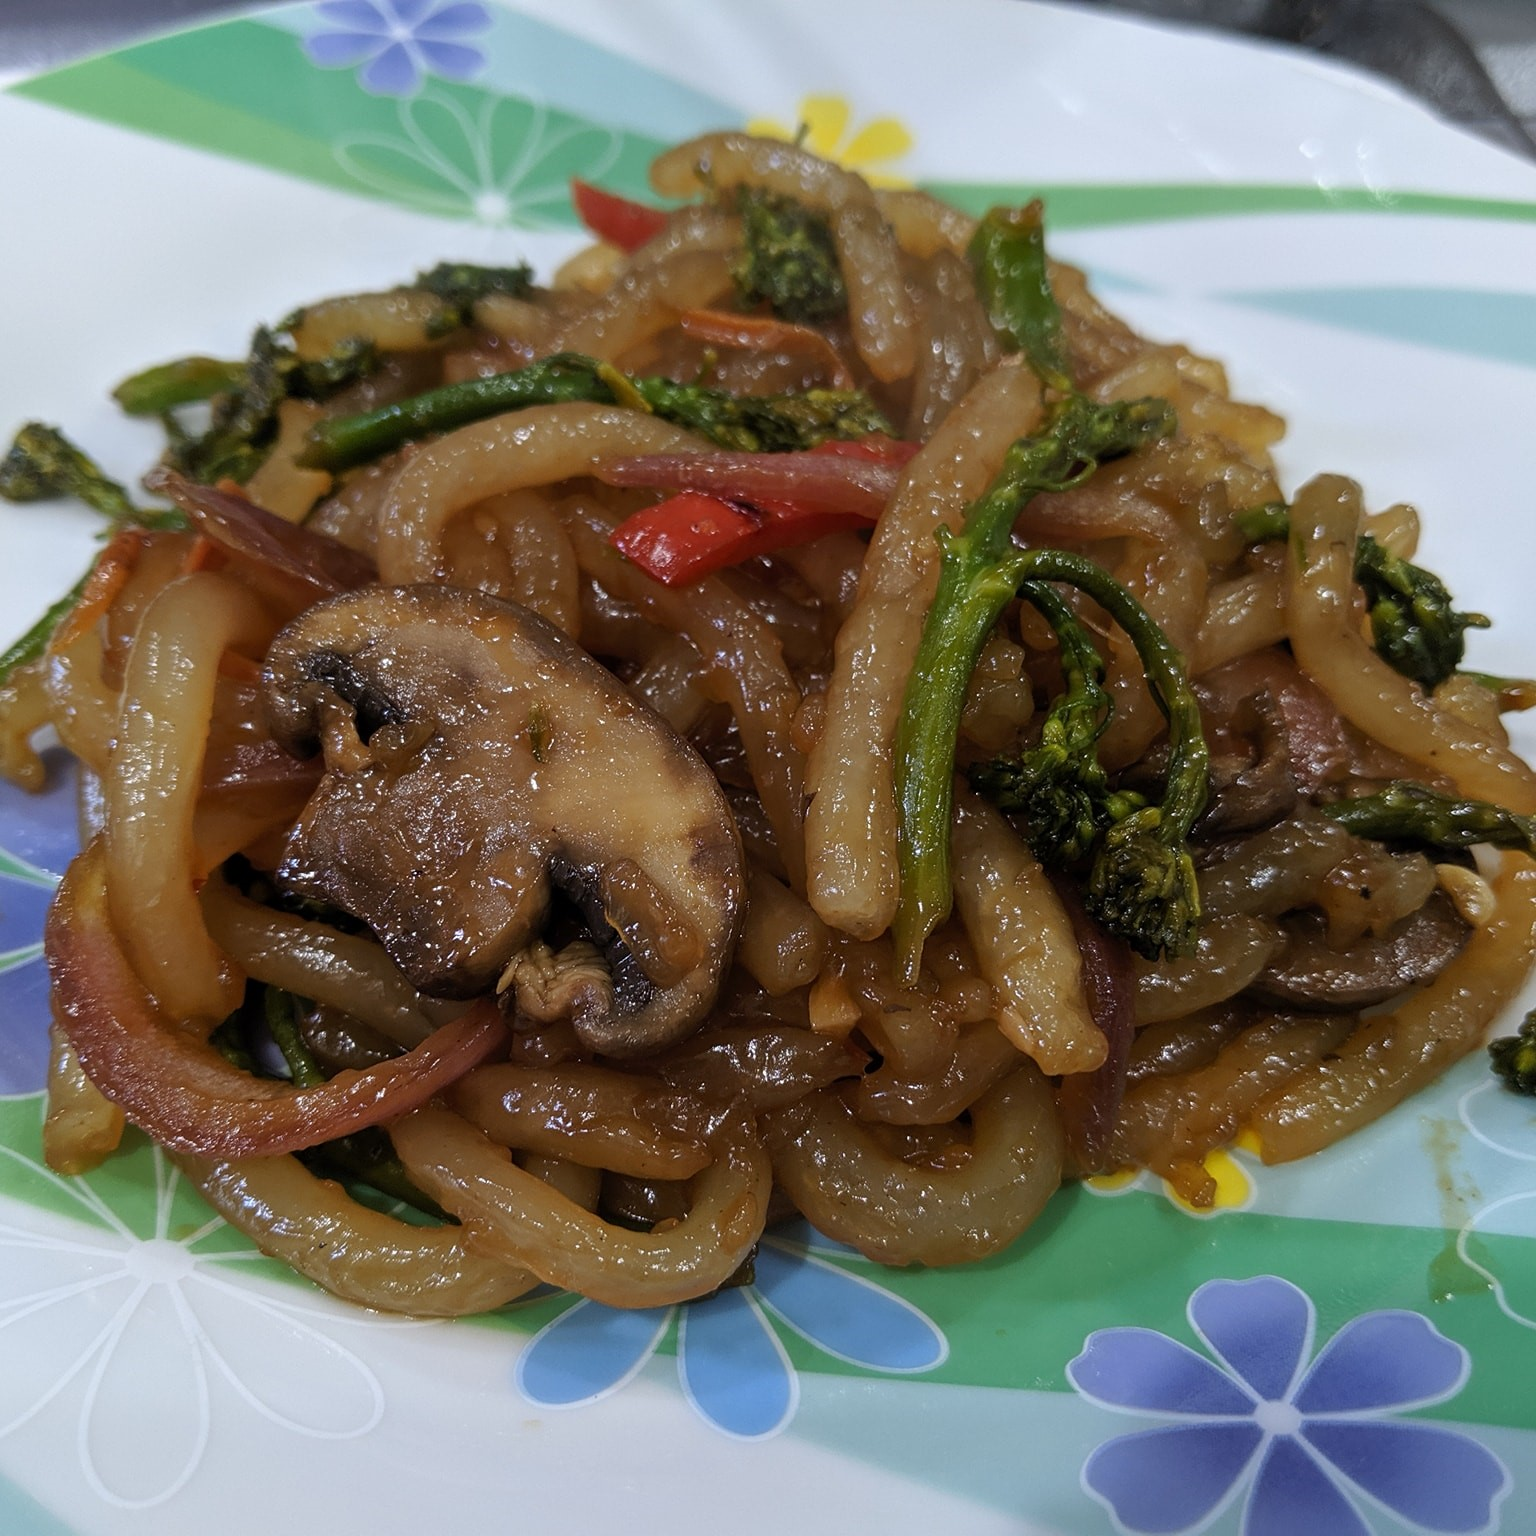
\includegraphics[width=0.15\textwidth]{sticky-udon-noodles}}}\end{floatingfigure}\begin{huge}Sticky Udon Noodles\end{huge}\newline\vspace{-2.5mm}\newline\renewcommand{\arraystretch}{1.1}\begin{tabular*}{\textwidth}{@{\extracolsep{\fill}}lr}Asian-inspired noodles and veggies with a warm tingle of spice\\Sunny C\end{tabular*}\newline\vspace{10mm}\newline\begin{huge}Ingredients\end{huge}\\\rule[2.8mm]{\textwidth}{.1pt}\vspace{-3mm}\begin{itemize}\item 30 oz fresh udon noodles\item 2 cups broccolini tops\item 1$\frac{1}{2}$ cups shiitake mushrooms, sliced\item 1 cup red onion, sliced\item 1 cup red bell pepper, sliced\item $\frac{1}{2}$ cup matchstick carrots\item 2 teas fresh ginger, minced\item 2 garlic cloves, minced\item $\frac{1}{2}$ cup low sodium soy sauce\item $\frac{1}{4}$ cup hoisin sauce\item 2 tbs mirin\item 2 tbs vegetable oil\item 2-3 teas sambal oelek\item Chopped green onions (optional, for topping)\item Mung bean sprouts (optional, for topping)\item Roasted black sesame seeds (optional, for topping)\end{itemize}\vspace{7mm}\begin{huge}Directions\end{huge}\\\rule[2.8mm]{\textwidth}{.1pt}\vspace{-3mm}\begin{enumerate}\item Combine soy sauce, hoisin sauce, mirin, sambal oelek, ginger, and garlic in a bowl. Whisk thoroughly and set aside.\item Cook udon noodles according to package directions. Meanwhile, add vegetable oil to wok or large pan and heat on medium-high for two minutes. Add veggies and sauté for three minutes.\item Add $\frac{1}{3}$ of soy sauce mixture and sauté an additional 2 minutes. Add noodles to veggies and pour remaining sauce over top. Sauté a minimum of 3 minutes, or until sauce is clinging to food and noodles are sticky.\end{enumerate}\end{document}